\begin{frame}
    \frametitle{Game - Definition}

    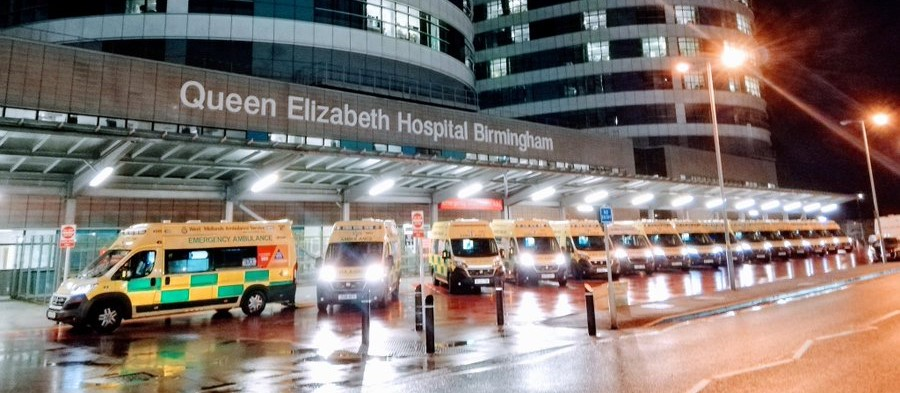
\includegraphics[scale=0.45]{Bin/ambulance_queue.jpg}

    \pause
    \footnotesize
    \begin{itemize}
        \item Misra S, Sarkar S. Priority-based time-slot allocation in wireless body area networks during medical emergency situations: An evolutionary game-theoretic perspective
        \item Song J, Wen J. A non-cooperative game with incomplete information to improve patient hospital choice
    \end{itemize}
\end{frame}

\begin{frame}
    \frametitle{Game - Players and objectives}

    \begin{minipage}{.35\textwidth}
        \begin{figure}
            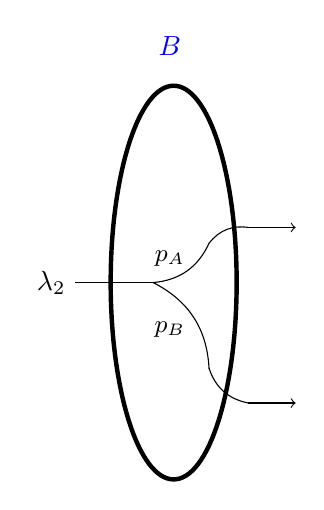
\begin{tikzpicture}
                \draw[ultra thick] (0.75,2) ellipse (0.8cm and 2.5cm);
                \node[blue] at (0.7, 5) {};
                \only<2>{
                    \node[blue] at (0.7, 5) {\( B \)};
                }
                \draw[-] (0.5, 2) -- ++(-1, 0) node[left] {\(\lambda_2\)};
                
                % p_A line
                \path (0.49, 2) edge [bend right=30] (1.2, 2.5);
                \path (1.2, 2.5) edge [bend left=30] (1.7, 2.7);
                \draw[->] (1.7, 2.7) -- ++(0.6, 0.);
                
                % p_B
                \path (0.49, 2) edge [bend left=30] (1.2, 0.9);
                \path (1.2, 0.91) edge [bend right=30] (1.7, 0.47);
                \draw[->] (1.7, 0.47) -- ++(0.6, 0.);


                \node at (0.7, 2.3) {\small{\( p_A \)}};
                \node at (0.7, 1.4) {\small{\( p_B \)}};

            \end{tikzpicture}
        \end{figure}
    \end{minipage}
    \begin{minipage}{.6\textwidth}
        \begin{figure}
            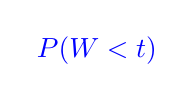
\begin{tikzpicture}
                \node[blue] at (0, 0) {};
                \only<2>{
                    \node[blue] at (0, 0) {\( P(W < t) \)};
                }
            \end{tikzpicture}
            \scalebox{.8}{
                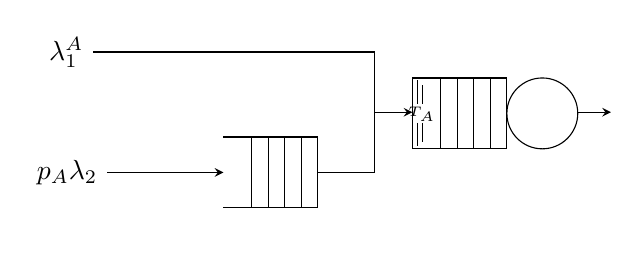
\begin{tikzpicture}[>=stealth, scale=0.6]
                    % the rectangle with vertical rules (Queue 1)
                    \draw (1,0) -- ++(2cm,0) -- ++(0,-1.5cm) -- ++(-2cm,0);
                    \foreach \i in {1,...,4}
                    \draw (3cm-\i*10pt,0) -- +(0,-1.5cm);
         
                    % the rectangle with vertical rules (Queue 2)
                    \draw (5,1.25) -- ++(2cm,0) -- ++(0,-1.5cm) -- ++(-2cm,0);
                    \foreach \i in {1,...,4, 5.7}
                    \draw (7cm-\i*10pt,1.25) -- +(0,-1.5cm);
    
                    % The two vertical lines at the very start of Queue 2 
                    \draw (7cm-54pt, 1.2) -- +(0, -0.5cm);
                    \draw (7cm-54pt, 0.3) -- +(0, -0.5cm);        
                    \draw (7cm-51pt, 1.1) -- +(0, -0.4cm);
                    \draw (7cm-51pt, 0.3) -- +(0, -0.4cm);
            
                    % The label between the lines for T
                    \node[anchor=north] at (5.2, 0.84) {\tiny{\( T_A \)}};
    
                    % the circle (Queue 2)
                    \draw (7.75,0.5) circle [radius=0.75cm];
            
                    % the arrows and labels (Queue 1+2)
                    \draw[->] (8.5,0.525) -- +(20pt,0);
                    \node[align=center] at (1cm,-2cm) {};
                    \node[align=center] at (6cm,-0.75cm) {};
                    
                    % Ambulance lines
                    \draw[<-] (1,-0.75) -- +(-70pt,0) node[left] {\( p_A \lambda_2 \)};
                    % \draw[-] (3.5,-0.75) -- +(20pt,0);
                    \draw[-] (3,-0.75) -- (4.2,-0.75);
                    \draw (4.2, 0.525) -- (4.2, -0.75);
    
                    % Others lines
                    \draw (4.2, 1.8) -- +(-169.5pt,0) node[left] {\( \lambda_1^A \)};
                    \draw (4.2, 1.8) -- (4.2, 0.525);
                    \draw[->] (4.2, 0.525) -- (5, 0.525);
                \end{tikzpicture}
            }
            \scalebox{.8}{
                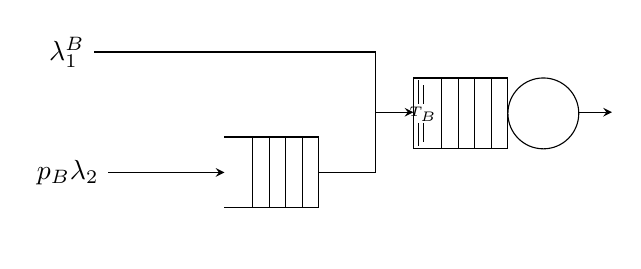
\begin{tikzpicture}[>=stealth, scale=0.6] %arrow type
                    % the rectangle with vertical rules (Queue 1)
                    \draw (1,0) -- ++(2cm,0) -- ++(0,-1.5cm) -- ++(-2cm,0);
                    \foreach \i in {1,...,4}
                    \draw (3cm-\i*10pt,0) -- +(0,-1.5cm);
                                
                    % the rectangle with vertical rules (Queue 2)
                    \draw (5,1.25) -- ++(2cm,0) -- ++(0,-1.5cm) -- ++(-2cm,0);
                    \foreach \i in {1,...,4, 5.7}
                    \draw (7cm-\i*10pt,1.25) -- +(0,-1.5cm);
    
                    % The two vertical lines at the very start of Queue 2 
                    \draw (7cm-54pt,1.2) -- +(0,-0.5cm);
                    \draw (7cm-54pt,0.3) -- +(0,-0.5cm);        
                    \draw (7cm-51pt,1.1) -- +(0,-0.4cm);
                    \draw (7cm-51pt,0.3) -- +(0,-0.4cm);
            
                    % The label between the lines for T
                    \node[anchor=north] at (5.2, 0.84) {\tiny{\( T_B \)}};
    
                    % the circle (Queue 2)
                    \draw (7.75,0.5) circle [radius=0.75cm];
            
                    % the arrows and labels (Queue 1+2)
                    \draw[->] (8.5,0.525) -- +(20pt,0);
                    \node[align=center] at (1cm,-2cm) {};
                    \node[align=center] at (6cm,-0.75cm) {};
                    
                    % Ambulance lines
                    \draw[<-] (1,-0.75) -- +(-70pt,0) node[left] {\( p_B \lambda_2 \)};
                    \draw[-] (3,-0.75) -- (4.2,-0.75);
                    \draw (4.2, 0.525) -- (4.2, -0.75);
    
                    % Others lines
                    \draw (4.2, 1.8) -- +(-169.5pt,0) node[left] {\( \lambda_1^B \)};
                    \draw (4.2, 1.8) -- (4.2, 0.525);
                    \draw[->] (4.2, 0.525) -- (5, 0.525);
                \end{tikzpicture}
            }
        \end{figure}
    \end{minipage}
\end{frame}


\begin{frame}
    \frametitle{Performance Measures - Blocking time}
    \centering
    \begin{equation*}
        B = \frac{\sum_{(u,v) \in S_A^{(2)}} \pi_{(u,v)} \; 
        b(u,v)}{\sum_{(u,v) \in S_A^{(2)}} \pi_{(u,v)}}
    \end{equation*}

\end{frame}


\begin{frame}
    \frametitle{Performance Measures - Blocking time}

    \scriptsize
    \begin{equation*}
        B = \frac{\sum_{(u,v) \in S_A^{(2)}} \pi_{(u,v)} \; 
        b(u,v)}{\sum_{(u,v) \in S_A^{(2)}} \pi_{(u,v)}}
    \end{equation*}

    \tiny
    \pause
    \begin{equation*}
        b(u,v) = 
        \begin{cases} 
            0, & \textbf{if } (u,v) \notin S_b \\
            c(u,v) + b(u - 1, v), & \textbf{if } v = N = T\\
            c(u,v) + b(u, v-1), & \textbf{if } v = N \neq T \\
            c(u,v) + p_s(u,v) b(u-1, v) + p_a(u,v) b(u, v+1), & \textbf{if } u > 0 
            \textbf{ and } \\ 
            & \quad v = T \\
            c(u,v) + p_s(u,v) b(u, v-1) + p_a(u,v) b(u, v+1), & \textbf{otherwise} \\
        \end{cases}
    \end{equation*}
    
    \begin{equation*}
        S_b = \{(u,v) \in S \; | \; u > 0\}
    \end{equation*}
        
    \begin{equation*}
        c(u,v) = 
        \begin{cases}
            \frac{1}{\min(v,C) \mu}, & \text{if } v = N\\
            \frac{1}{\lambda_1 + \min(v,C) \mu}, & \text{otherwise}
        \end{cases}
    \end{equation*}
    
    \begin{equation*}
        p_s(u,v) = \frac{\min(v,C)\mu}{\lambda_1 + \min(v,C)\mu}, \qquad
        p_a(u,v) = \frac{\lambda_1}{\lambda_1 + \min(v,C)\mu}
    \end{equation*}
    
\end{frame}


\begin{frame}
    \frametitle{Performance Measures - Proportion within time}
    \centering
    
    \small
    \begin{equation*}
        P(W < t) = \frac{\lambda_1 P_{L'_1}}{\lambda_2 P_{L'_2}+\lambda_1 P_{L'_1}} 
        P(W^{(1)} < t) + \frac{\lambda_2 P_{L'_2}}{\lambda_2 P_{L'_2} + 
        \lambda_1 P_{L'_1}}P(W^{(2)} < t) 
    \end{equation*}

    \begin{equation*}
        P(W^{(1)} < t) = \frac{\sum_{(u,v) \in S_A^{(1)}} P(W_{(u,v)}^{(1)} < t) 
        \pi_{u,v} }{\sum_{(u,v) \in S_A^{(1)}} \pi_{u,v}}
    \end{equation*}
    
    
    \begin{equation*}
        P(W^{(2)} < t) = \frac{\sum_{(u,v) \in S_A^{(2)}} P(W_{(u,v)}^{(2)} < t) 
        \pi_{u,v} }{\sum_{(u,v) \in S_A^{(2)}} \pi_{u,v}}
    \end{equation*}
    
\end{frame}


\begin{frame}
    \frametitle{Performance Measures - Proportion within time}

    \scriptsize
    \begin{equation*}
        P(W^{(i)} < t) = \frac{\sum_{(u,v) \in S_A^{(i)}} P(W_{u,v}^{(i)} < t) 
        \pi_{u,v} }{\sum_{(u,v) \in S_A^{(i)}} \pi_{u,v}}, \quad \textbf{for } i = \{1, 2\}
    \end{equation*}

    \only<1>{
        \vspace{6.15cm}
    }
    
    \pause
    \only<3>{
        \tiny
        \vspace{0.9cm}
        \begin{equation*}
            P(W_{(u,v)}^{(1)} < t) = 
            \begin{cases}
                1 - \sum_{i=0}^{v-1} \frac{1}{i!} e^{-\mu t} (\mu t)^i, 
                & \textbf{if } C = 1 \textbf{ and } v>1 \\
                1 - (\mu C)^{v-C} \mu  
                    \sum_{k=1}^{\mid \vec{r} \mid} \sum_{l=1}^{r_k}
                    \frac{\Psi_{k,l}(-\lambda_k)t^{r_k - l} 
                    e^{-\lambda_k t}}{(r_k - l)! (l - 1)!},
                & \textbf{if } C > 1 \textbf{ and } v > C \\
                    \qquad \textbf{where } \vec{r}=(v - C, 1) \textbf{ and } 
                    \vec{\lambda}=(C \mu, \mu) &  \\
                1 - e^{-\mu t},  & \textbf{if } v \leq C
            \end{cases}
        \end{equation*}
        \vspace{0.9cm}
        \begin{equation*}
            P(W_{(u,v)}^{(2)} < t) = 
            \begin{cases}
                1 - \sum_{i=0}^{\min(v,T)-1} \frac{1}{i!} e^{-\mu t} (\mu t)^i,  
                & \textbf{if } C = 1 \textbf{ and } v, T > 1 \\
                1 - \mu (\mu C) ^ {\min(v,T) - C} 
                    \sum_{k=1}^{\mid \vec{r} \mid} \sum_{l=1}^{r_k} 
                    \frac{\Psi_{k,l}(-\lambda_k)t^{r_k - l} 
                    e^{-\lambda_k t}}{(r_k - l)! (l - 1)!}, 
                & \textbf{if } C > 1 \textbf{ and } v, T  > C \\
                    \qquad \textbf{where } \vec{r}=(\min(v, T) - C, 1) 
                    \textbf{ and } \vec{\lambda}=(C \mu, \mu) \\
                1 - e^{-\mu t}, & \textbf{if } v \leq C 
                    \textbf{ or } T \leq C \\
            \end{cases}
        \end{equation*}
        \vspace{0.85cm}
    }
    
    \only<2>{
        \vspace{1cm}
        \begin{equation*}
            W_{(u,v)}^{(1)} \sim 
            \begin{cases}
                \textbf{Erlang}(v, \mu), & \textbf{if } C = 1 \textbf{ and } v>1 \\
                \textbf{Hypo} \left(
                    \left[v - C, 1\right], \left[C \mu, \mu \right]
                \right), & \textbf{if } C > 1 \textbf{ and } v>C \\
                \textbf{Erlang}(1, \mu), & \textbf{if } v \leq C
            \end{cases}
        \end{equation*}
        \vspace{1cm}
        \begin{equation*}
            W_{(u,v)}^{(2)} \sim 
            \begin{cases}
                \textbf{Erlang}(\min(v, T), \mu), & \textbf{if } C = 1
                    \textbf{ and } v, T > 1 \\
                \textbf{Hypo}\left(
                    \left[ \min(v, T) - C, 1 \right], \left[ C \mu, \mu \right]
                \right), & \textbf{if } C > 1 \textbf{ and } v, T  > C \\
                \textbf{Erlang}(1, \mu), & \textbf{if } v \leq C \textbf{ or } T \leq C
            \end{cases}
        \end{equation*}
        \vspace{1cm}
    }
    

\end{frame}


\begin{frame}
    \frametitle{Comparisons}

    \setlength{\columnseprule}{1pt}
    \begin{multicols}{3}
        \centering
        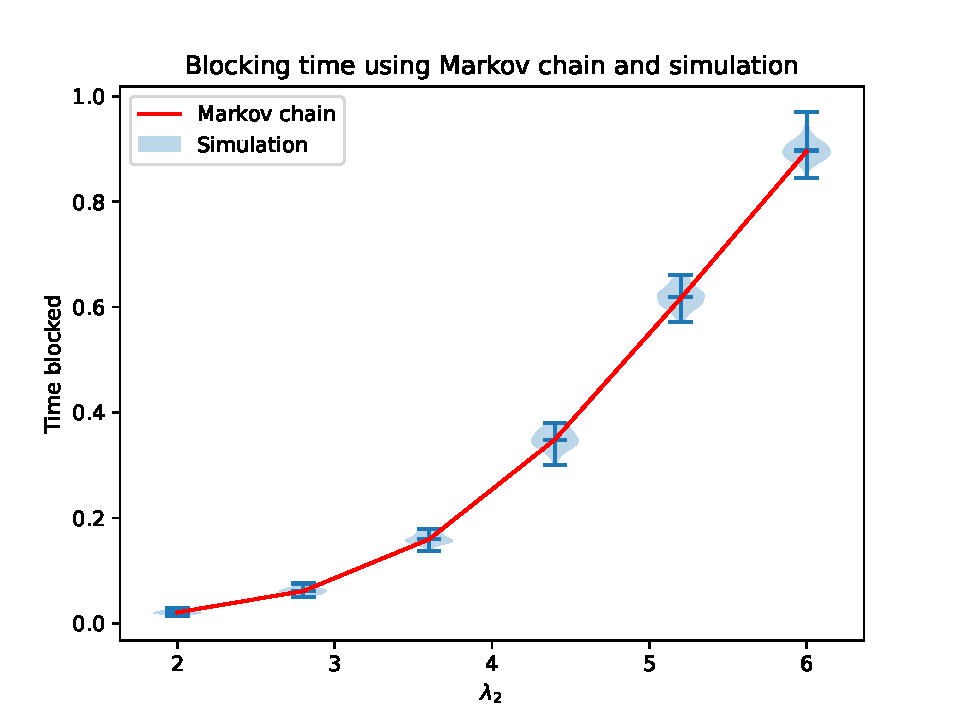
\includegraphics[scale=0.2]{Bin/performance_measures_comparison/blocking_comparison.pdf}

        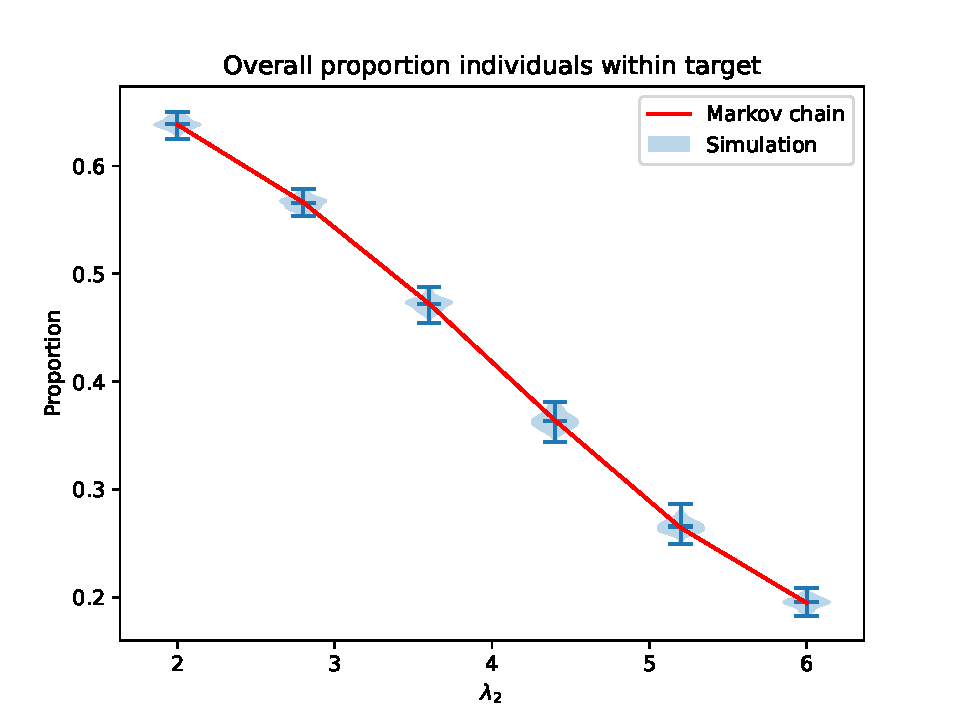
\includegraphics[scale=0.2]{Bin/performance_measures_comparison/proportion_overall_comparison.pdf}
        
        \columnbreak

        \centering
        \vspace*{0.05cm}
        \Huge{\, N/A}
        \vspace{0.75cm}

        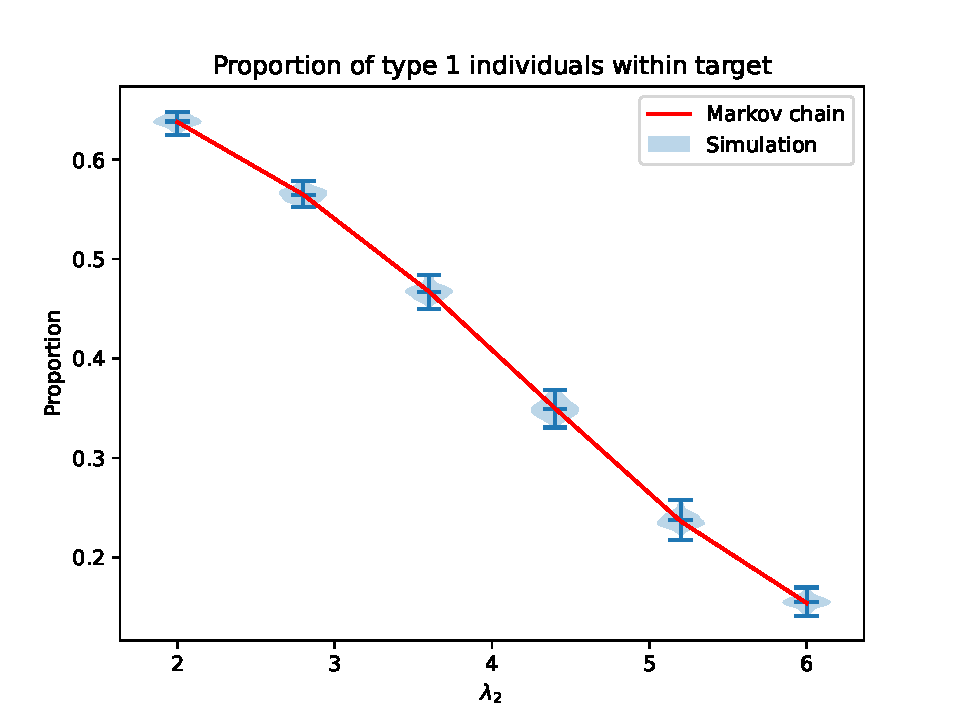
\includegraphics[scale=0.2]{Bin/performance_measures_comparison/proportion_1_comparison.pdf}
        
        \columnbreak
        \centering
        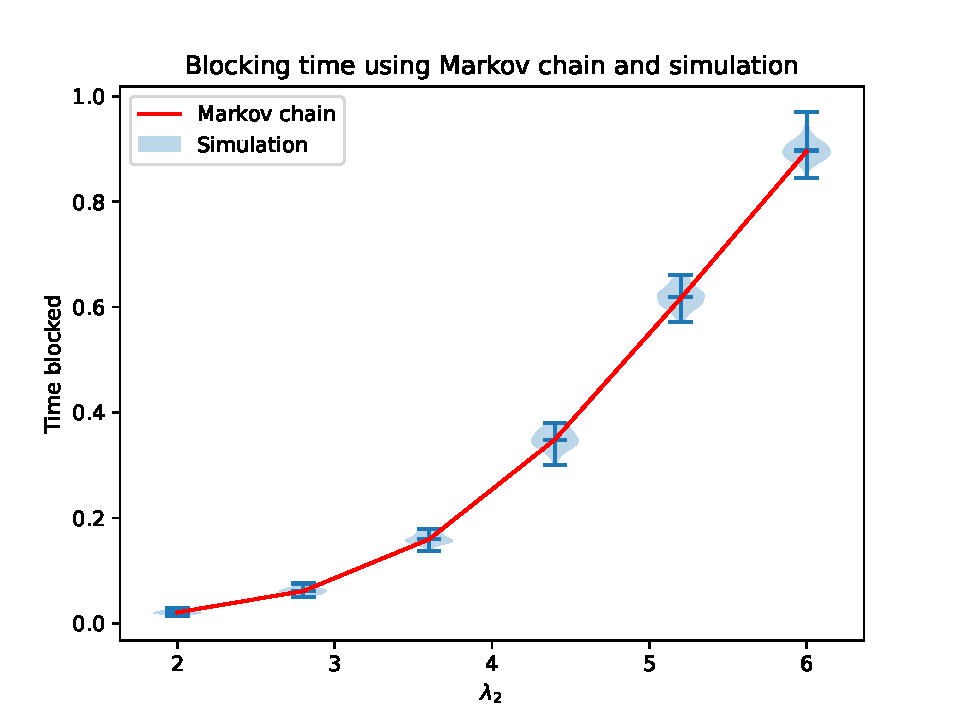
\includegraphics[scale=0.2]{Bin/performance_measures_comparison/blocking_comparison.pdf}
        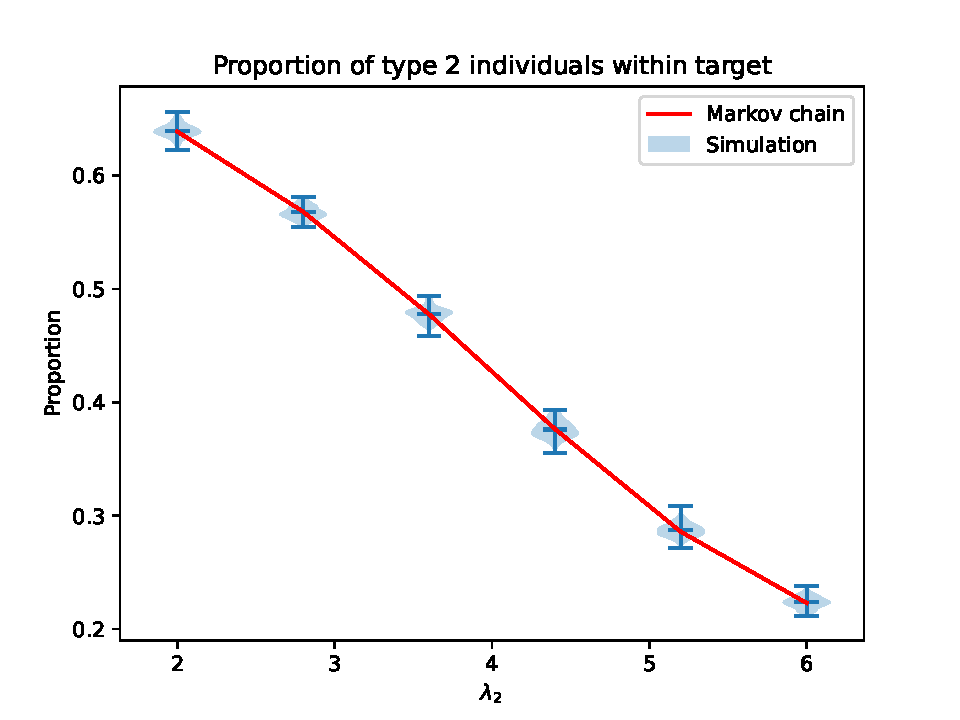
\includegraphics[scale=0.2]{Bin/performance_measures_comparison/proportion_2_comparison.pdf}
    \end{multicols}


\end{frame}